\documentclass[11pt]{article}
\usepackage[letterpaper,margin=0.9in]{geometry}
\usepackage{amsmath,amssymb}
\usepackage{booktabs}
\usepackage[T1]{fontenc}
\usepackage{lmodern}
\usepackage{microtype}
\usepackage{graphicx}
\usepackage{placeins}
\usepackage[hidelinks]{hyperref}
\setlength{\parindent}{0pt}
\setlength{\parskip}{0.45em}
\newcommand{\MASK}{\ensuremath{?\!?}}
\newcommand{\PAD}{\ensuremath{\square}}

\title{NLP Assignment 2: Solutions}
\author{PAN CHANGXUN\\Student ID: 2024011323}
\date{November 2026}

\begin{document}
\maketitle
\vspace{-2em}

\section*{Part 1: Pretrain Transformer}

\subsection*{(b) Model}

A decoder-only Transformer (GPT style) with
4 layers, 8 attention heads, embedding size 256 (32 per head),
block size 128, and a character vocabulary of 256 symbols
(3{,}323{,}392 parameters).
Each block uses pre-norm residual connections,
\[
x \leftarrow x + \mathrm{Attn}(\mathrm{LN}_1(x)),\qquad
x \leftarrow x + \mathrm{MLP}(\mathrm{LN}_2(x)),
\]
where the MLP is $\mathrm{Linear}(256,1024)\to\mathrm{GELU}\to\mathrm{Linear}(1024,256)\to\mathrm{Dropout}$.
Attention is scaled dot-product attention with a causal mask, filled with
$-\infty$ before the softmax.
The loss is the cross-entropy (log-softmax + NLL) over all positions,
ignoring the padding character (\texttt{ignore\_index=0}).
Dropout is 0.1 everywhere.

% TODO (optional): one or two sentences on why you chose pre-norm,
% or on the role of the causal mask.

\subsection*{(c) Finetuning without pretraining}

Trained on \texttt{birth\_places\_train.tsv} (2000 examples) from random
initialisation: 75 epochs, batch size 256, learning rate $6\times10^{-4}$
with linear warm-up and cosine decay. Training loss went from 3.49 to 0.31.

\begin{center}
\begin{tabular}{lc}
\toprule
 & Dev accuracy \\
\midrule
Finetune without pretraining & \textbf{2.0\%} (10 / 500) \\
Always predict ``London'' & 5.0\% (25 / 500) \\
\bottomrule
\end{tabular}
\end{center}

The model's most frequent predictions were London (53), Paris (21) and
Chicago (18), the most common birthplaces in the training set.

% TODO: explain in your own words why accuracy is this low. Points to cover:
% the dev people never appear in the finetuning data; the training loss is low
% but the model is memorising; it falls back to frequent places, and does no
% better than the trivial London baseline.

\subsection*{(d) Pretraining with span corruption}

\texttt{CharCorruptionDataset.\_\_getitem\_\_} builds each example as follows:
\begin{enumerate}
  \item Take document \texttt{idx} and truncate it to a random length
        $L\in[4,\min(112,\,|\text{doc}|)]$, keeping its beginning.
  \item Draw a span length $m\in[1,\lfloor L/2\rfloor-1]$ (mean $\approx L/4$)
        and a start position $s\in[0,L-m]$, splitting the text into
        prefix, masked content and suffix.
  \item Form \texttt{prefix \MASK{} suffix \MASK{} masked \MASK{}} and pad with \PAD{}
        to length 129; then $x$ is the string without its last character
        and $y$ the string without its first.
\end{enumerate}
Over 5 passes of the corpus (14{,}685 samples) the measured truncation lengths
covered the full range 4--112 and the masked span averaged 24.4\% of the
truncated text.

Pretraining: 650 epochs on \texttt{wiki.txt}, batch size 128, learning rate
$6\times10^{-3}$ with warm-up and cosine decay. It was run on a GPU
(RTX 5080) and finished in under 20 minutes. Training loss:

\begin{center}
\begin{tabular}{cccccc}
\toprule
Epoch & 1 & 100 & 300 & 500 & 650 \\
\midrule
Loss & 3.45 & 1.40 & 0.81 & 0.58 & 0.52 \\
\bottomrule
\end{tabular}
\end{center}

% TODO: explain the design choices in your own words: why the third MASK
% matches the finetuning format "question MASK place MASK"; why truncating
% from the start keeps the name and birthplace in the same window.

\subsection*{(e) Finetuning the pretrained model}

Starting from the pretrained weights: 10 epochs, batch size 256, learning rate
$6\times10^{-4}$. Training loss went from 0.78 (epoch 1) to 0.16 (epoch 10).

\begin{center}
\begin{tabular}{lc}
\toprule
 & Dev accuracy \\
\midrule
Finetune without pretraining & 2.0\% (10 / 500) \\
Pretrain, then finetune & \textbf{24.4\%} (122 / 500) \\
\bottomrule
\end{tabular}
\end{center}

Examples that only the pretrained model answers correctly:

\begin{center}
\begin{tabular}{llll}
\toprule
Person & Gold & Without pretraining & With pretraining \\
\midrule
Ralf Wadephul & Berlin & Paris & Berlin \\
Joseph Baggaley & England & Boston & England \\
Alfred Mele & Detroit & England & Detroit \\
Ernst Florian Winter & Vienna & Dallas & Vienna \\
\bottomrule
\end{tabular}
\end{center}

% TODO: analysis in your own words: where the knowledge comes from (these
% people appear in wiki.txt but not in the finetuning data); what pretraining
% teaches versus what finetuning teaches; why the first-epoch loss is already
% much lower; and why accuracy is still far from 100%.

\section*{Part 3: SFT and RL}

All experiments were run locally on one RTX 5080 (16\,GB) under WSL2 (Ubuntu 24.04),
with LLaMA-Factory (SFT), lighteval + vLLM (evaluation) and verl (GRPO).

\textbf{Experiment logs (SwanLab, public):}
\url{https://swanlab.cn/@Anthropic/NLP2026_2024011323}.
SwanLab is used instead of wandb, as permitted by the instructor.
The runs were executed with local logging only (LLaMA-Factory \texttt{trainer\_log.jsonl},
lighteval result files, verl's file logger); the recorded metrics were afterwards
uploaded to SwanLab by a replay script, one run per task
(\texttt{TASK\_3\_1\_1}--\texttt{TASK\_3\_1\_4}, \texttt{TASK\_3\_2\_1}), all tagged
\texttt{replayed-from-local-logs}. The curves and numbers are the original ones;
only the upload time and system monitoring differ from a live run.

\subsection*{3-1 SFT}

\textbf{Evaluation setting.} \texttt{lighteval|gsm8k|5} (5-shot, 1319 test problems),
vLLM backend, bf16, \texttt{max\_model\_length=4096},
\texttt{max\_new\_tokens=4096}, temperature 0.6, top-$p$ 0.95, metric
\texttt{extractive\_match}. The same setting is used for every model.

\textbf{Training setting.} Full-parameter SFT of Qwen2.5-0.5B-Instruct, Qwen chat
template, bf16, learning rate $10^{-5}$ with cosine decay, effective batch size 32,
gradient checkpointing.

\begin{center}
\begin{tabular}{llc}
\toprule
Task & Model & GSM8K (5-shot) \\
\midrule
(a) & Qwen2.5-0.5B-Instruct & 38.21\% $\pm$ 1.34 \\
(b) & + SFT on \texttt{alpaca\_en\_demo} & 33.89\% $\pm$ 1.30 \\
(c)/(d) & + SFT on OpenMathInstruct-2 subset (ours) & \textbf{48.45\%} $\pm$ 1.38 \\
\bottomrule
\end{tabular}
\end{center}

\subsubsection*{(a) Base model}
Qwen2.5-0.5B-Instruct scores \textbf{38.21\%} on GSM8K (run \texttt{TASK\_3\_1\_1}).

\subsubsection*{(b) SFT on alpaca\_en\_demo}
1000 examples, 3 epochs (96 optimizer steps), batch $2\times16$ (gradient accumulation),
cutoff length 2048, warm-up ratio 0.1. Training took 73 minutes.
The loss falls from 1.35 to about 0.75 (Figure~\ref{fig:sft}, left).
The finetuned model scores 33.89\% on GSM8K.

% TODO: in your own words: why the loss drops at each epoch boundary
% (steps 32 and 64), and why general instruction data does not help
% (and here slightly hurts) GSM8K.

\subsubsection*{(c) Our dataset: a GSM8K-style subset of OpenMathInstruct-2}
We streamed the \texttt{train\_1M} split of \texttt{nvidia/OpenMathInstruct-2} and kept
an example only if
\begin{enumerate}
  \item its \texttt{problem\_source} is \texttt{gsm8k} or \texttt{augmented\_gsm8k},
        so the problems match the style and difficulty of the target benchmark;
  \item the generated solution contains a final \verb|\boxed{}| answer;
  \item the solution is at most 1500 characters, which keeps short, direct
        step-by-step solutions and fits the 1024-token cutoff;
  \item its problem text has not been seen before (deduplication by problem).
\end{enumerate}
We stopped after 20{,}000 examples and converted them to alpaca format
(\texttt{instruction} = problem, \texttt{output} = solution).
Training: 2 epochs (1250 optimizer steps), batch $1\times32$, cutoff length 1024,
warm-up ratio 0.05, 78 minutes. The loss falls from 0.64 to about 0.26
(Figure~\ref{fig:sft}, right).

\begin{figure}[h]
\centering
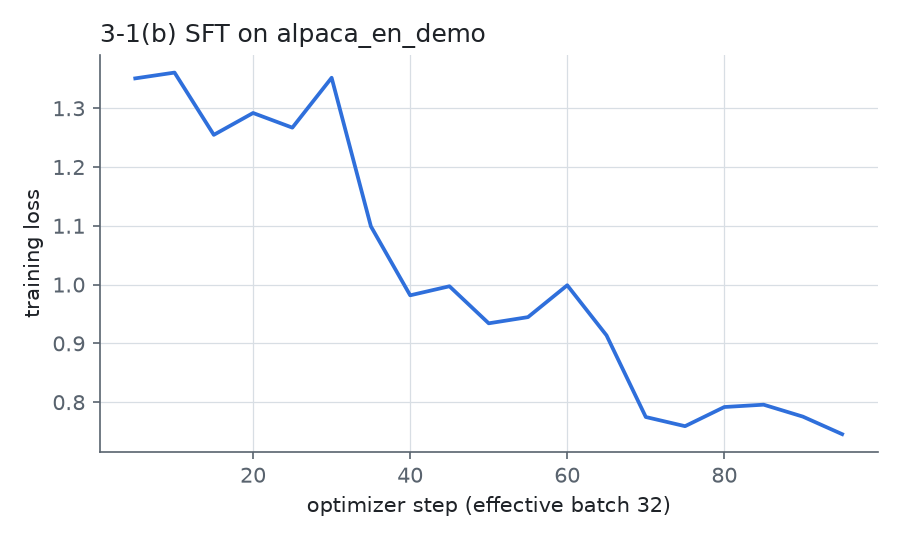
\includegraphics[width=0.49\linewidth]{figs/task_3_1_2_loss.png}\hfill
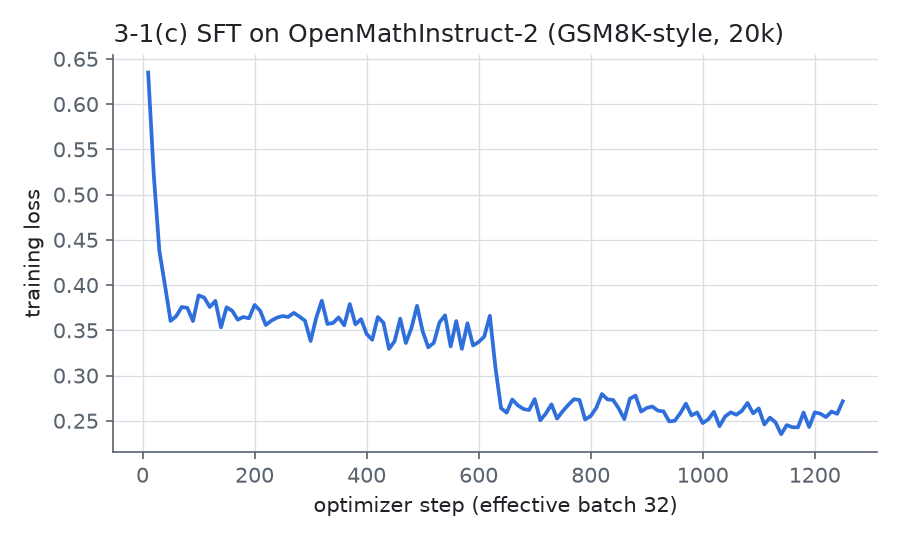
\includegraphics[width=0.49\linewidth]{figs/task_3_1_3_loss.png}
\caption{Training loss of 3-1(b) (left, run \texttt{TASK\_3\_1\_2}) and
3-1(c) (right, run \texttt{TASK\_3\_1\_3}).}
\label{fig:sft}
\end{figure}

\subsubsection*{(d) Evaluation of the finetuned model}
With the same evaluation setting as in (a), the model from (c) scores
\textbf{48.45\%} on GSM8K, \textbf{+10.2} points over the base model
(run \texttt{TASK\_3\_1\_4}).

% TODO: in your own words: why task-matched math data helps while alpaca did not;
% what the step in the loss at the start of epoch 2 (~step 625) means.

\subsection*{3-2 RL: GRPO on Qwen2.5-0.5B}

\textbf{Data.} Subset \texttt{simplelr\_qwen\_gsm8k\_level1} of
\texttt{hkust-nlp/SimpleRL-Zoo-Data} (GSM8K + MATH level 1, the setting SimpleRL-Zoo uses
for its 0.5B model). We sampled 2000 training problems and 200 problems of its MATH500
test split for validation (6 of them have prompts longer than 256 tokens and are
filtered, leaving 194). Each prompt ends with ``Please reason step by step, and put your
final answer within \verb|\boxed{}|.''

\textbf{Reward.} Rule-based: 1 if the last \verb|\boxed{}| answer matches the reference
(verl's MATH scorer), otherwise 0.

\textbf{Setup.} verl, GRPO advantage estimator, base model Qwen2.5-0.5B (not Instruct).
32 prompts per step with $n=8$ sampled responses each, learning rate $10^{-6}$,
mini-batch 32 (one update per step), max prompt / response length 256 / 768 tokens,
no KL loss and no entropy bonus, 2 epochs = 124 steps. Validation every 10 steps with
greedy decoding. The run took about 3 hours (about 85\,s per step).

\begin{center}
\begin{tabular}{lll}
\toprule
Metric & Start & End \\
\midrule
Training reward (mean of 10 steps) & 0.073 & 0.611 \\
Validation accuracy (greedy) & 0.113 (step 0) & 0.284 (step 124), peak 0.320 (step 100) \\
Mean response length (tokens) & $\approx$390 & $\approx$320 \\
\bottomrule
\end{tabular}
\end{center}

\begin{figure}[h]
\centering
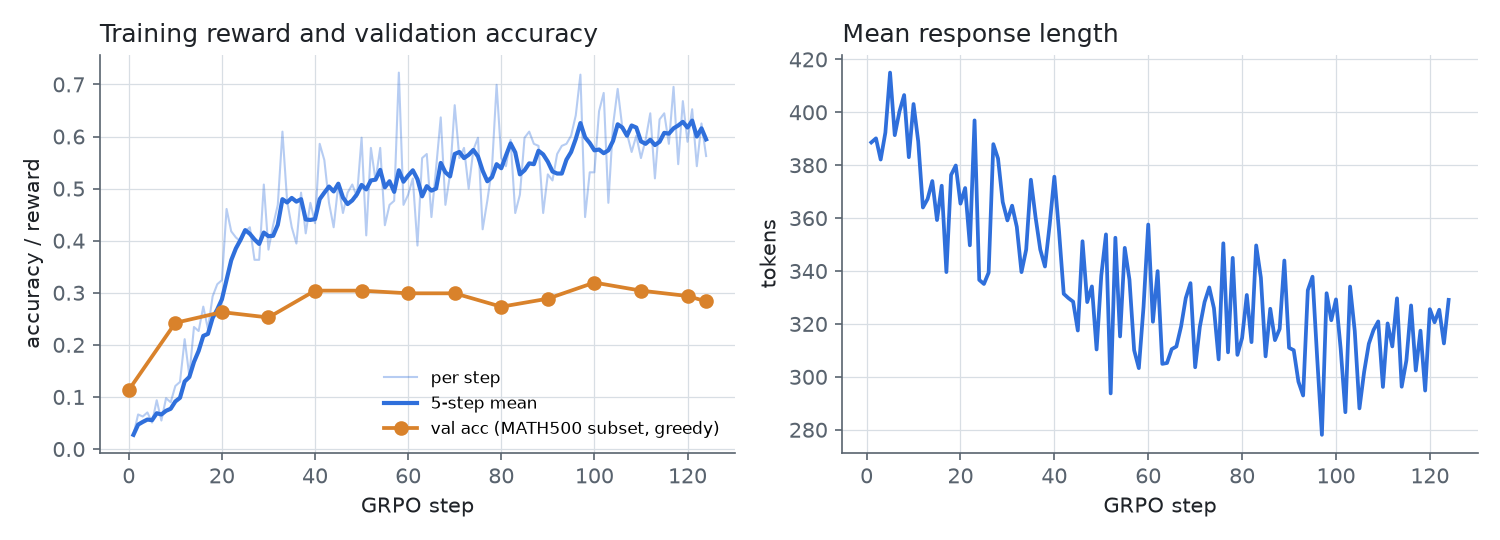
\includegraphics[width=\linewidth]{figs/grpo_curves.png}
\caption{GRPO training (run \texttt{TASK\_3\_2\_1}). Left: training reward (accuracy
of the sampled responses) and validation accuracy on the MATH500 subset. Right: mean
response length.}
\label{fig:grpo}
\end{figure}

Training reward rises from 7\% to about 60\%, and validation accuracy rises from
11.3\% to about 30\%, reproducing the increasing-accuracy trend reported in
SimpleRL-Zoo.

% TODO: in your own words: why most of the gain happens in the first ~20 steps
% (the base model learns to give a \boxed{} answer and stop); why validation plateaus
% around 30% while the training reward keeps rising (training set much easier than
% MATH500, small model, small data); why the response length goes down instead of up
% (compare with SimpleRL-Zoo's observations on small models).
% Note the simplifications made for a 16GB GPU: no KL term / reference model,
% responses capped at 768 tokens (about 20% were truncated early in training).

\FloatBarrier
\section*{Acknowledgements and use of AI}

% TODO: list collaborators and online sources (framework repos/docs, datasets),
% and state honestly how and how much AI was used, as the guidelines require.

\end{document}
